\documentclass{article}
\usepackage{blindtext}
\usepackage[a4paper, total={6in, 9.4in}]{geometry}
\usepackage{indentfirst}
\usepackage{wrapfig}
\usepackage{graphicx}
\usepackage{mathtext}
\usepackage{amsmath}
\usepackage{siunitx} % Required for alignment
\usepackage{subfigure}
\usepackage{multirow}
\usepackage{rotating}
\usepackage{afterpage}
\usepackage[T1,T2A]{fontenc}
\usepackage[russian]{babel}
\usepackage{caption}
\usepackage[arrowdel]{physics}
\usepackage{booktabs}

\graphicspath{{pictures/}}

\title{\begin{center}Лабораторная работа №4.7.2\end{center}
Эффект Поккельса}
\author{Гёлецян А.Г.}
\date{\today}

\begin{document}

\pagenumbering{gobble}
\maketitle
\newpage
\pagenumbering{arabic}

\textbf{Цель работы:} Исследовать интерференцию рассеянного света, про-
шедшего кристалл; наблюдать изменение характера поляризации све-
та при наложении на кристалл электрического поля.

\section{Теоретическая часть}
\subsection{Интерференционные кольца при прохождении света через одноосный кристалл}
\begin{figure}[h]
    \center\includegraphics[width = 0.8\linewidth]{ustanovka_kolca.png}
    \caption{Схема для наблюдения интерференционной картины}\label{fig:ustanovka_kolca}
\end{figure}

При прохождении света через одноосный кристалл, показатель преломления необыкновенной
волны зависит от угла между направлением распространения волны и осью кристалла
по формуле

\begin{equation}
    \frac{1}{n_2^2} = \frac{\cos^2 \theta}{n_o^2} + \frac{\sin^2 \theta}{n_e^2}
    \label{eq:pokazatel_prelomlenia}
\end{equation}

Если считать, что $(n_o - n_e) \ll n_o$, то при малых углах $\theta$ можно
воспользоваться приближенной формулой

\begin{equation}
    n_2 \approx n_o - (n_o - n_e) \theta^2
    \label{eq:pokazatel_prelomlenia_approx}
\end{equation}

Показатель преломления обыкновенного луча не зависит от направления распространения:
$n_1 = n_o$. Если длине кристалла $l$, то после прохождения через кристалл между
обыкновенным и необыкновенным лучом набегает разность фаз

\begin{equation}
    \Delta \varphi = \frac{2\pi}{\lambda} l (n_1 - n_2) \approx
    \frac{2\pi}{\lambda} l (n_o - n_e) \theta^2
    \label{eq:raznost_faz}
\end{equation}

Для случая, когда разрешенное направление анализатора перпендикулярно направлению
поляризации лазера, условием для темного кольца с номером $m$ является
$\varphi = 2\pi m$, откуда следует

\begin{equation}
    \theta_m^2 = \frac{\lambda m}{l(n_o - n_e)}
    \label{eq:theta_m}
\end{equation}

При выхоже из кристалла луч преломляется на границе кристалл-воздух, поэтому угол
$\theta_{внешн} \approx n_o \theta$. Радиус $m$-го темного кольца
$r_m = L\theta_{внешн, m}$. Для квадрата радиуса

\begin{equation}
    r_m^2 = \frac{\lambda}{l} \frac{{(n_o L)}^2}{(n_o - n_e)} m
    \label{eq:r_m}
\end{equation}

\newpage
\subsection{Эффект Поккельса}

\begin{wrapfigure}{l}{0.4\textwidth}
  \begin{center}
    \includegraphics[width=0.38\textwidth]{pokkels_axes.png}
  \end{center}
  \caption{Главные оси при наличии напряжения вдоль $x$}\label{fig:pokkels_axes}
\end{wrapfigure}

При наличии электрического поля вдоль $x$ в кристалле появляются новые перпендикулярные
главные направления, показатели преломления которых равны $n_o \pm \Delta n$, где
$\Delta n = A \cdot E_{x}$. Пусть поляризация лазера вертикальна, а разрешенное
направление анализатора горизонтальна. Тогда, интенсивность света на выходе
будет зависеть от прикладываемого напряжения ($U = E_x d$) по закону

\begin{equation}
    I = I_0 \sin^2\left(\frac{\pi}{2}\frac{U}{U_{\lambda/2}}\right)
    \label{eq:pokkels}
\end{equation}

где
\begin{equation}
    U_{\lambda/2} = \frac{\lambda}{4A} \frac{d}{l}
    \label{eq:poluvolnovoe_napryajenie}
\end{equation}

\vspace{1cm}
\section{Измерения}
\subsection{Интерференционные кольца}
\begin{figure}[h]
    \center\includegraphics[width = 0.5\linewidth]{kolca.jpg}
    \caption{Интерференционные кольца}\label{fig:kolca}
\end{figure}

\begin{table}[h]
\begin{center}
\begin{tabular}{cr}
\toprule
 № кольца &  r, см \\
\midrule
 1 & 2.5 \\
 2 & 3.6 \\
 3 & 4.3 \\
 4 & 4.9 \\
 5 & 5.5 \\\midrule
 6 & 6.1 \\
 7 & 6.5 \\
 8 & 6.9 \\
 9 & 7.2 \\
\bottomrule
\end{tabular}
\caption{Зависимость радиусов темных колец от номера колец}
\end{center}
\end{table}

\newpage

\begin{figure}[h]
    \center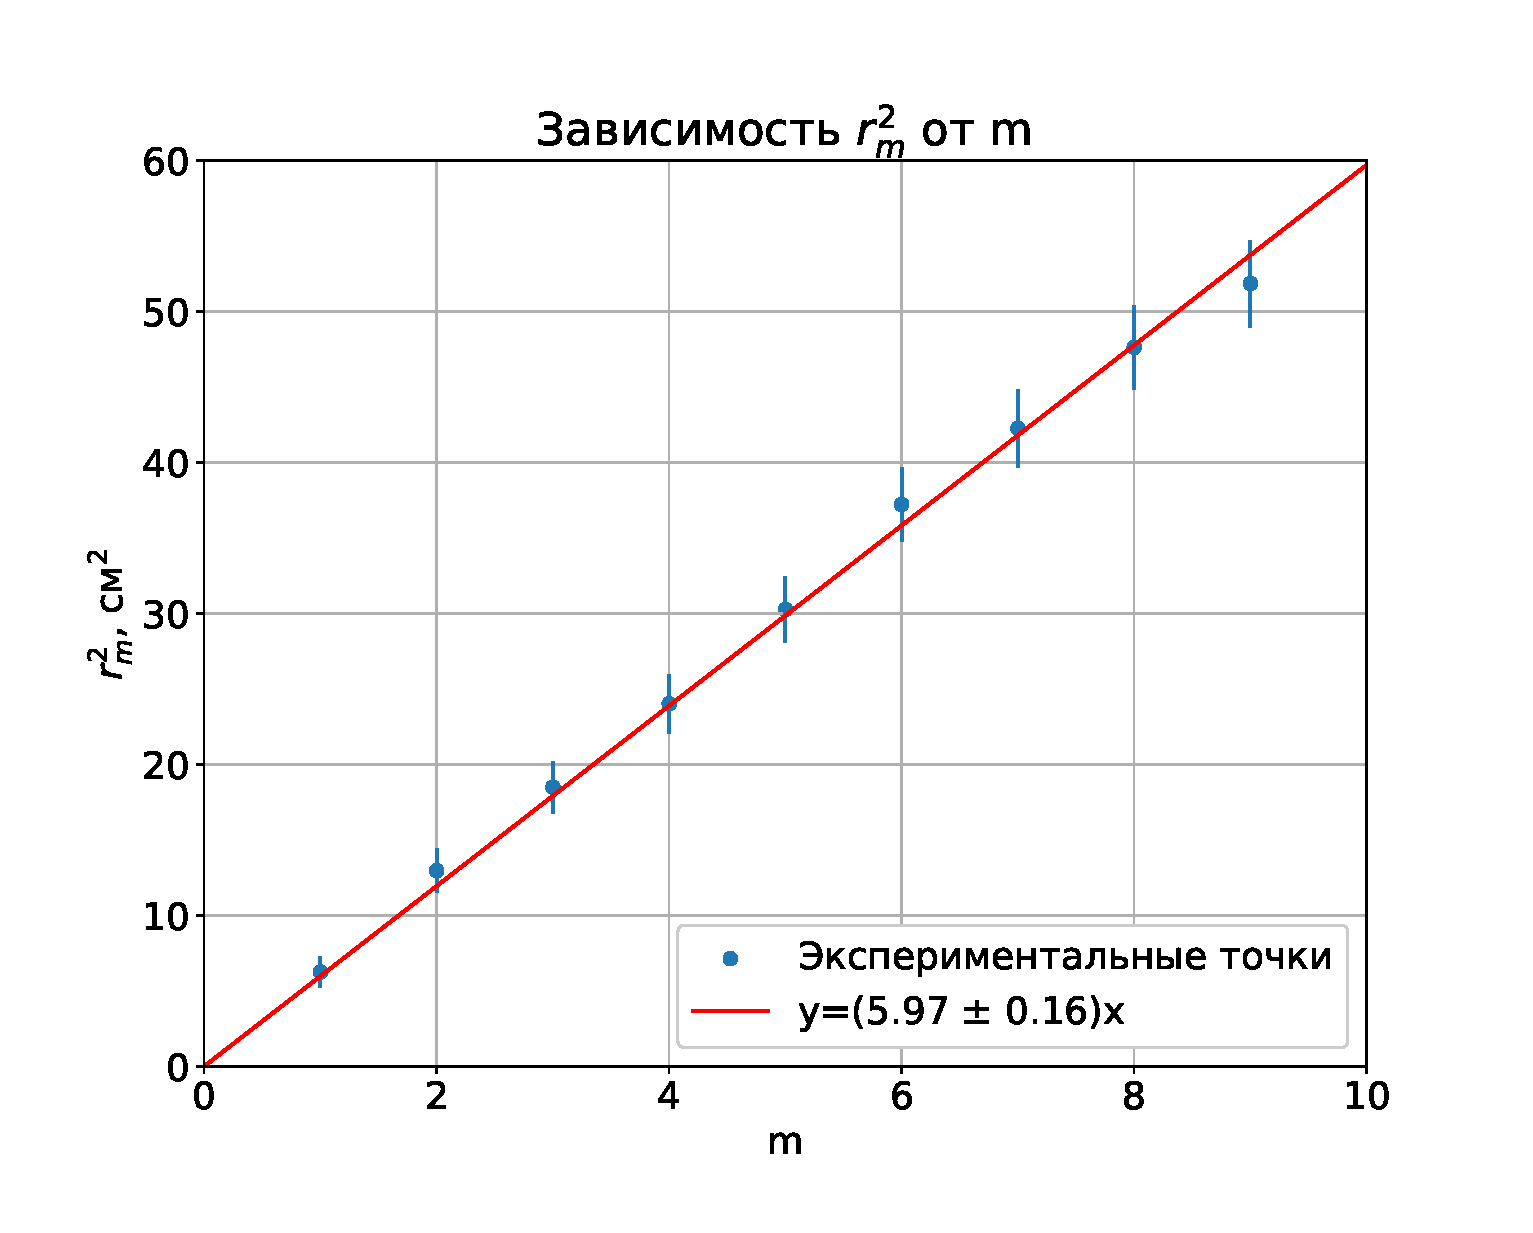
\includegraphics[width = 0.9\linewidth]{r_m.eps}
    \caption{Линеаризованные график зависимости радиуса колец от номера}\label{fig:r_m}
\end{figure}

Из графика и согласно формуле (\ref{eq:r_m})

\begin{equation*}
    \frac{\lambda}{l} \frac{{(n_o L)}^2}{(n_o - n_e)} = (5.97 \pm 0.16) \text{ см}^2
\end{equation*}

Для нашей установки $\lambda = 6328$ \AA, $l = 26$ мм, $L = (65.5 \pm 0.5)$ см,
$n_o = 2.29$. После подстановки получаем

\begin{equation}
    n_o - n_e = (0.092 \pm 0.003)
\end{equation}

\subsection{Эффект Поккельса}

\begin{table}[h]
\begin{center}
\begin{tabular}{ccc}
\toprule
Напряжение, В & скрещенные поляризации & парралельные поляризации\\
\midrule
U$_{\lambda/2}$ & 450 & 450\\
U$_{\lambda}$ & 900 & 900 \\
U$_{3\lambda/2}$ & 1350 & 1350\\
\bottomrule
\end{tabular}
\caption{Полуволновые, волновые и 3/2-волновые напряжения}
\end{center}
\end{table}

\newpage
\begin{figure}[h]
    \begin{center}
        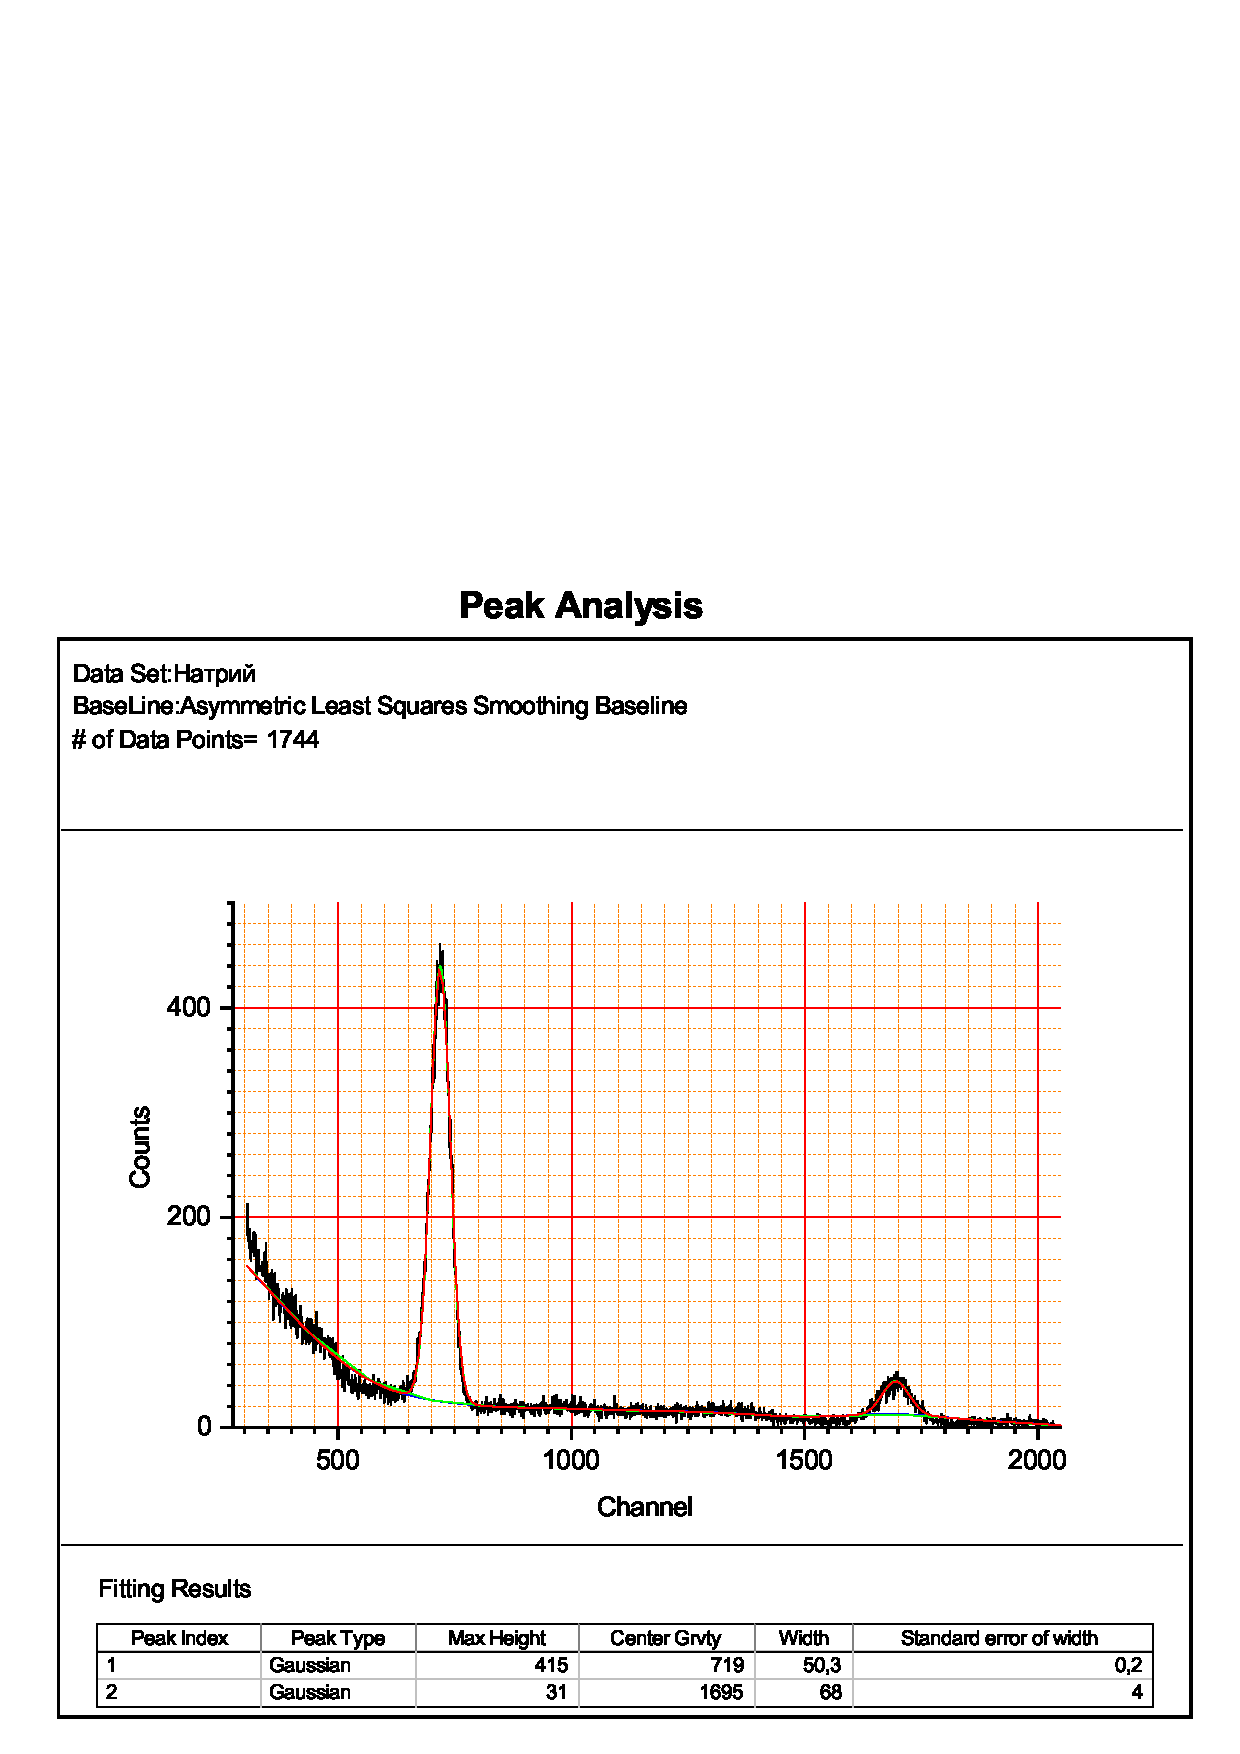
\includegraphics[width = 0.3\linewidth]{1.jpg}
        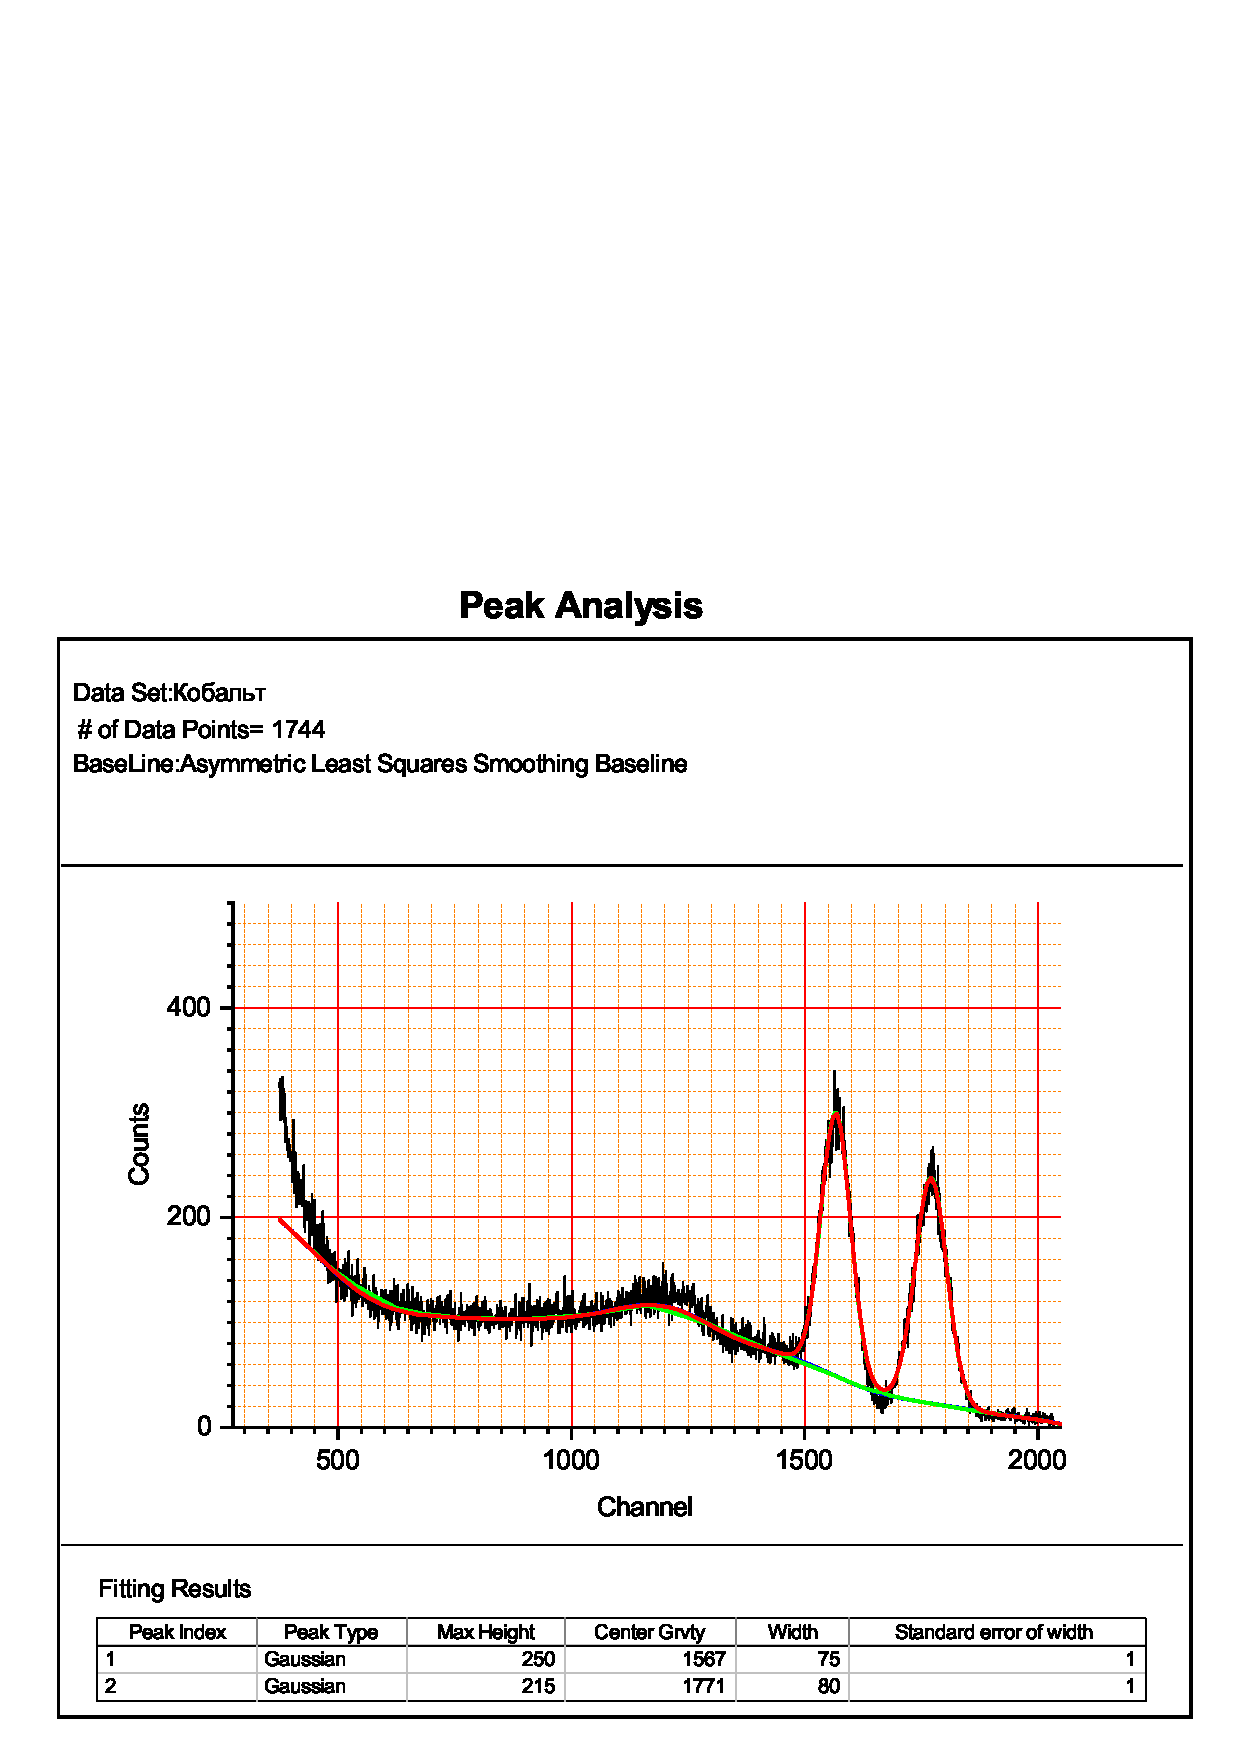
\includegraphics[width = 0.3\linewidth]{2.jpg}
        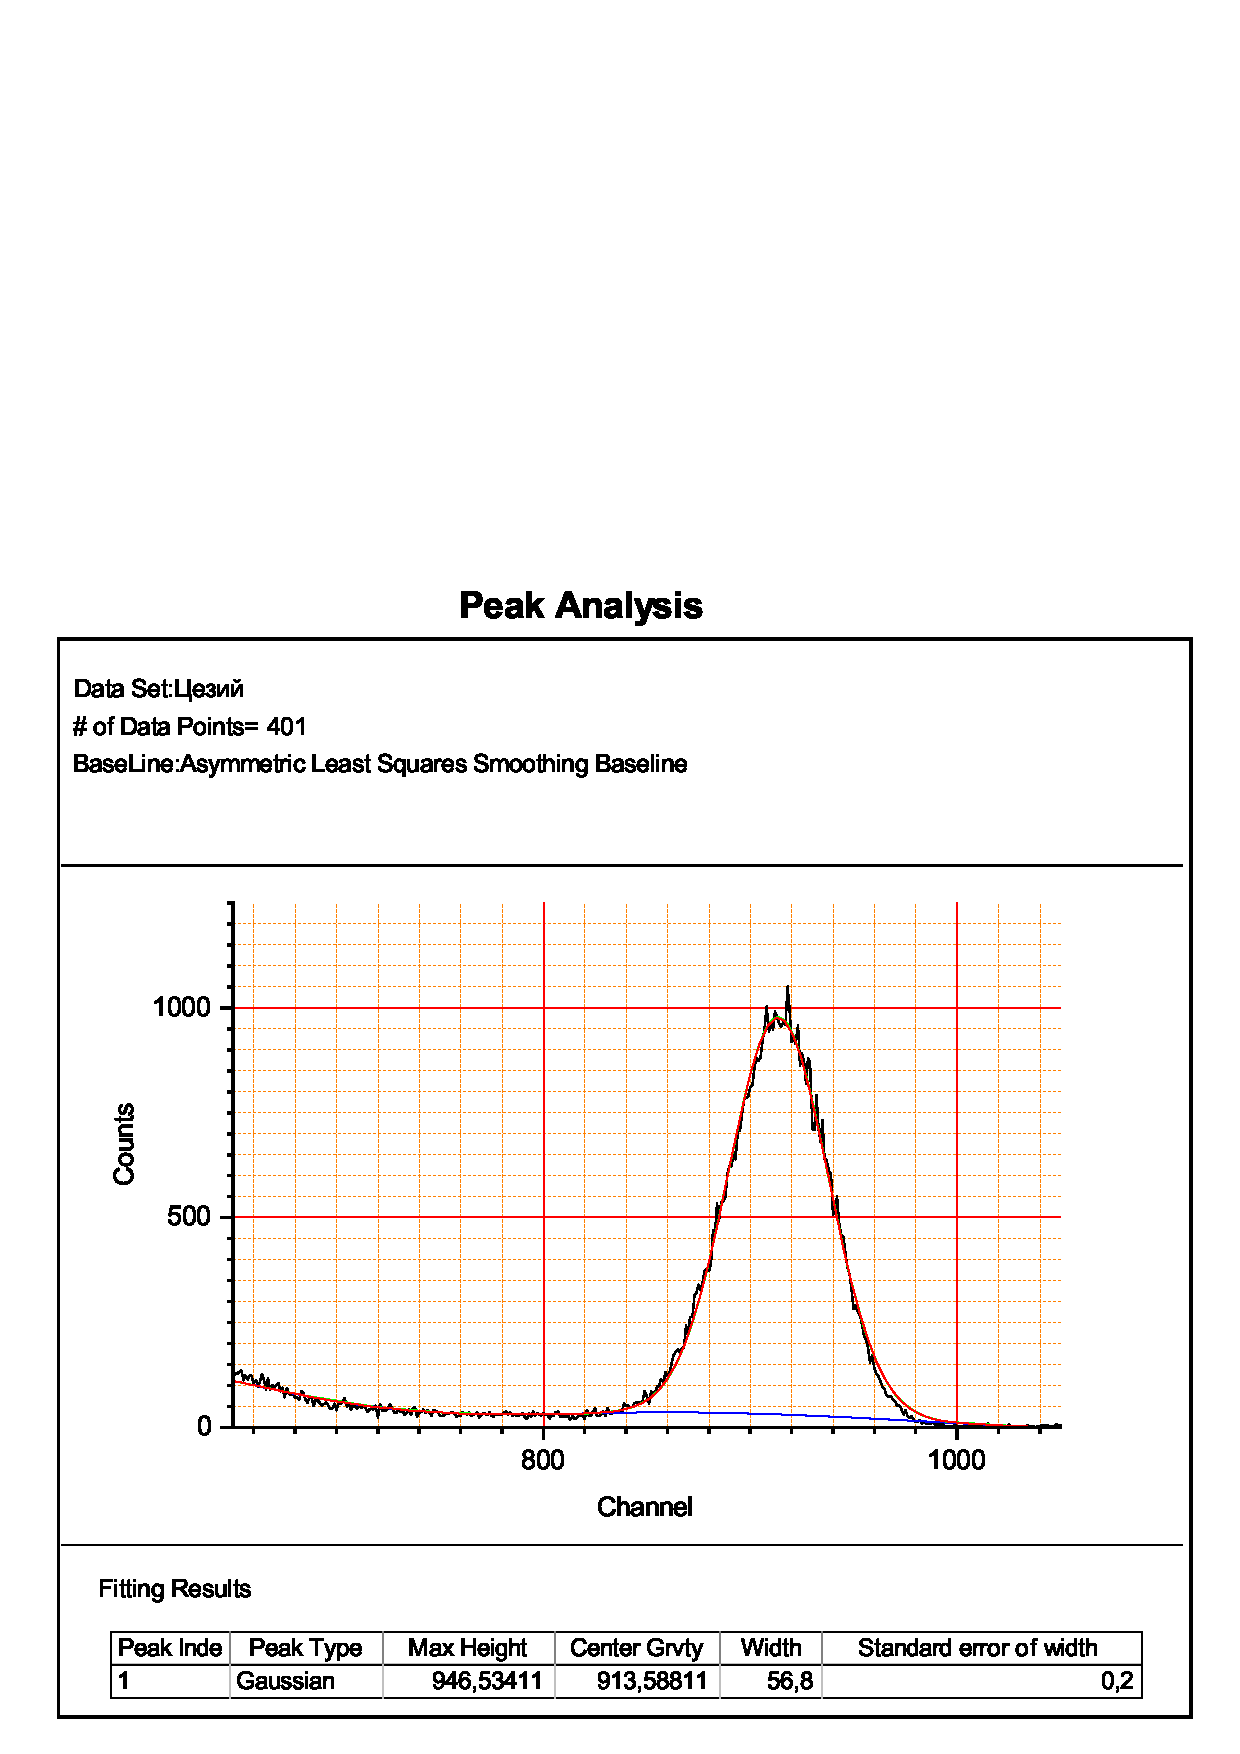
\includegraphics[width = 0.3\linewidth]{3.jpg}
    \end{center}
    \caption{Фигуры лиссажу для U$_{\lambda/2}$, U$_{\lambda}$ и U$_{3\lambda/2}$}
\end{figure}

\end{document}
